\begin{frame}{Introduction}
	\begin{figure}
		\centering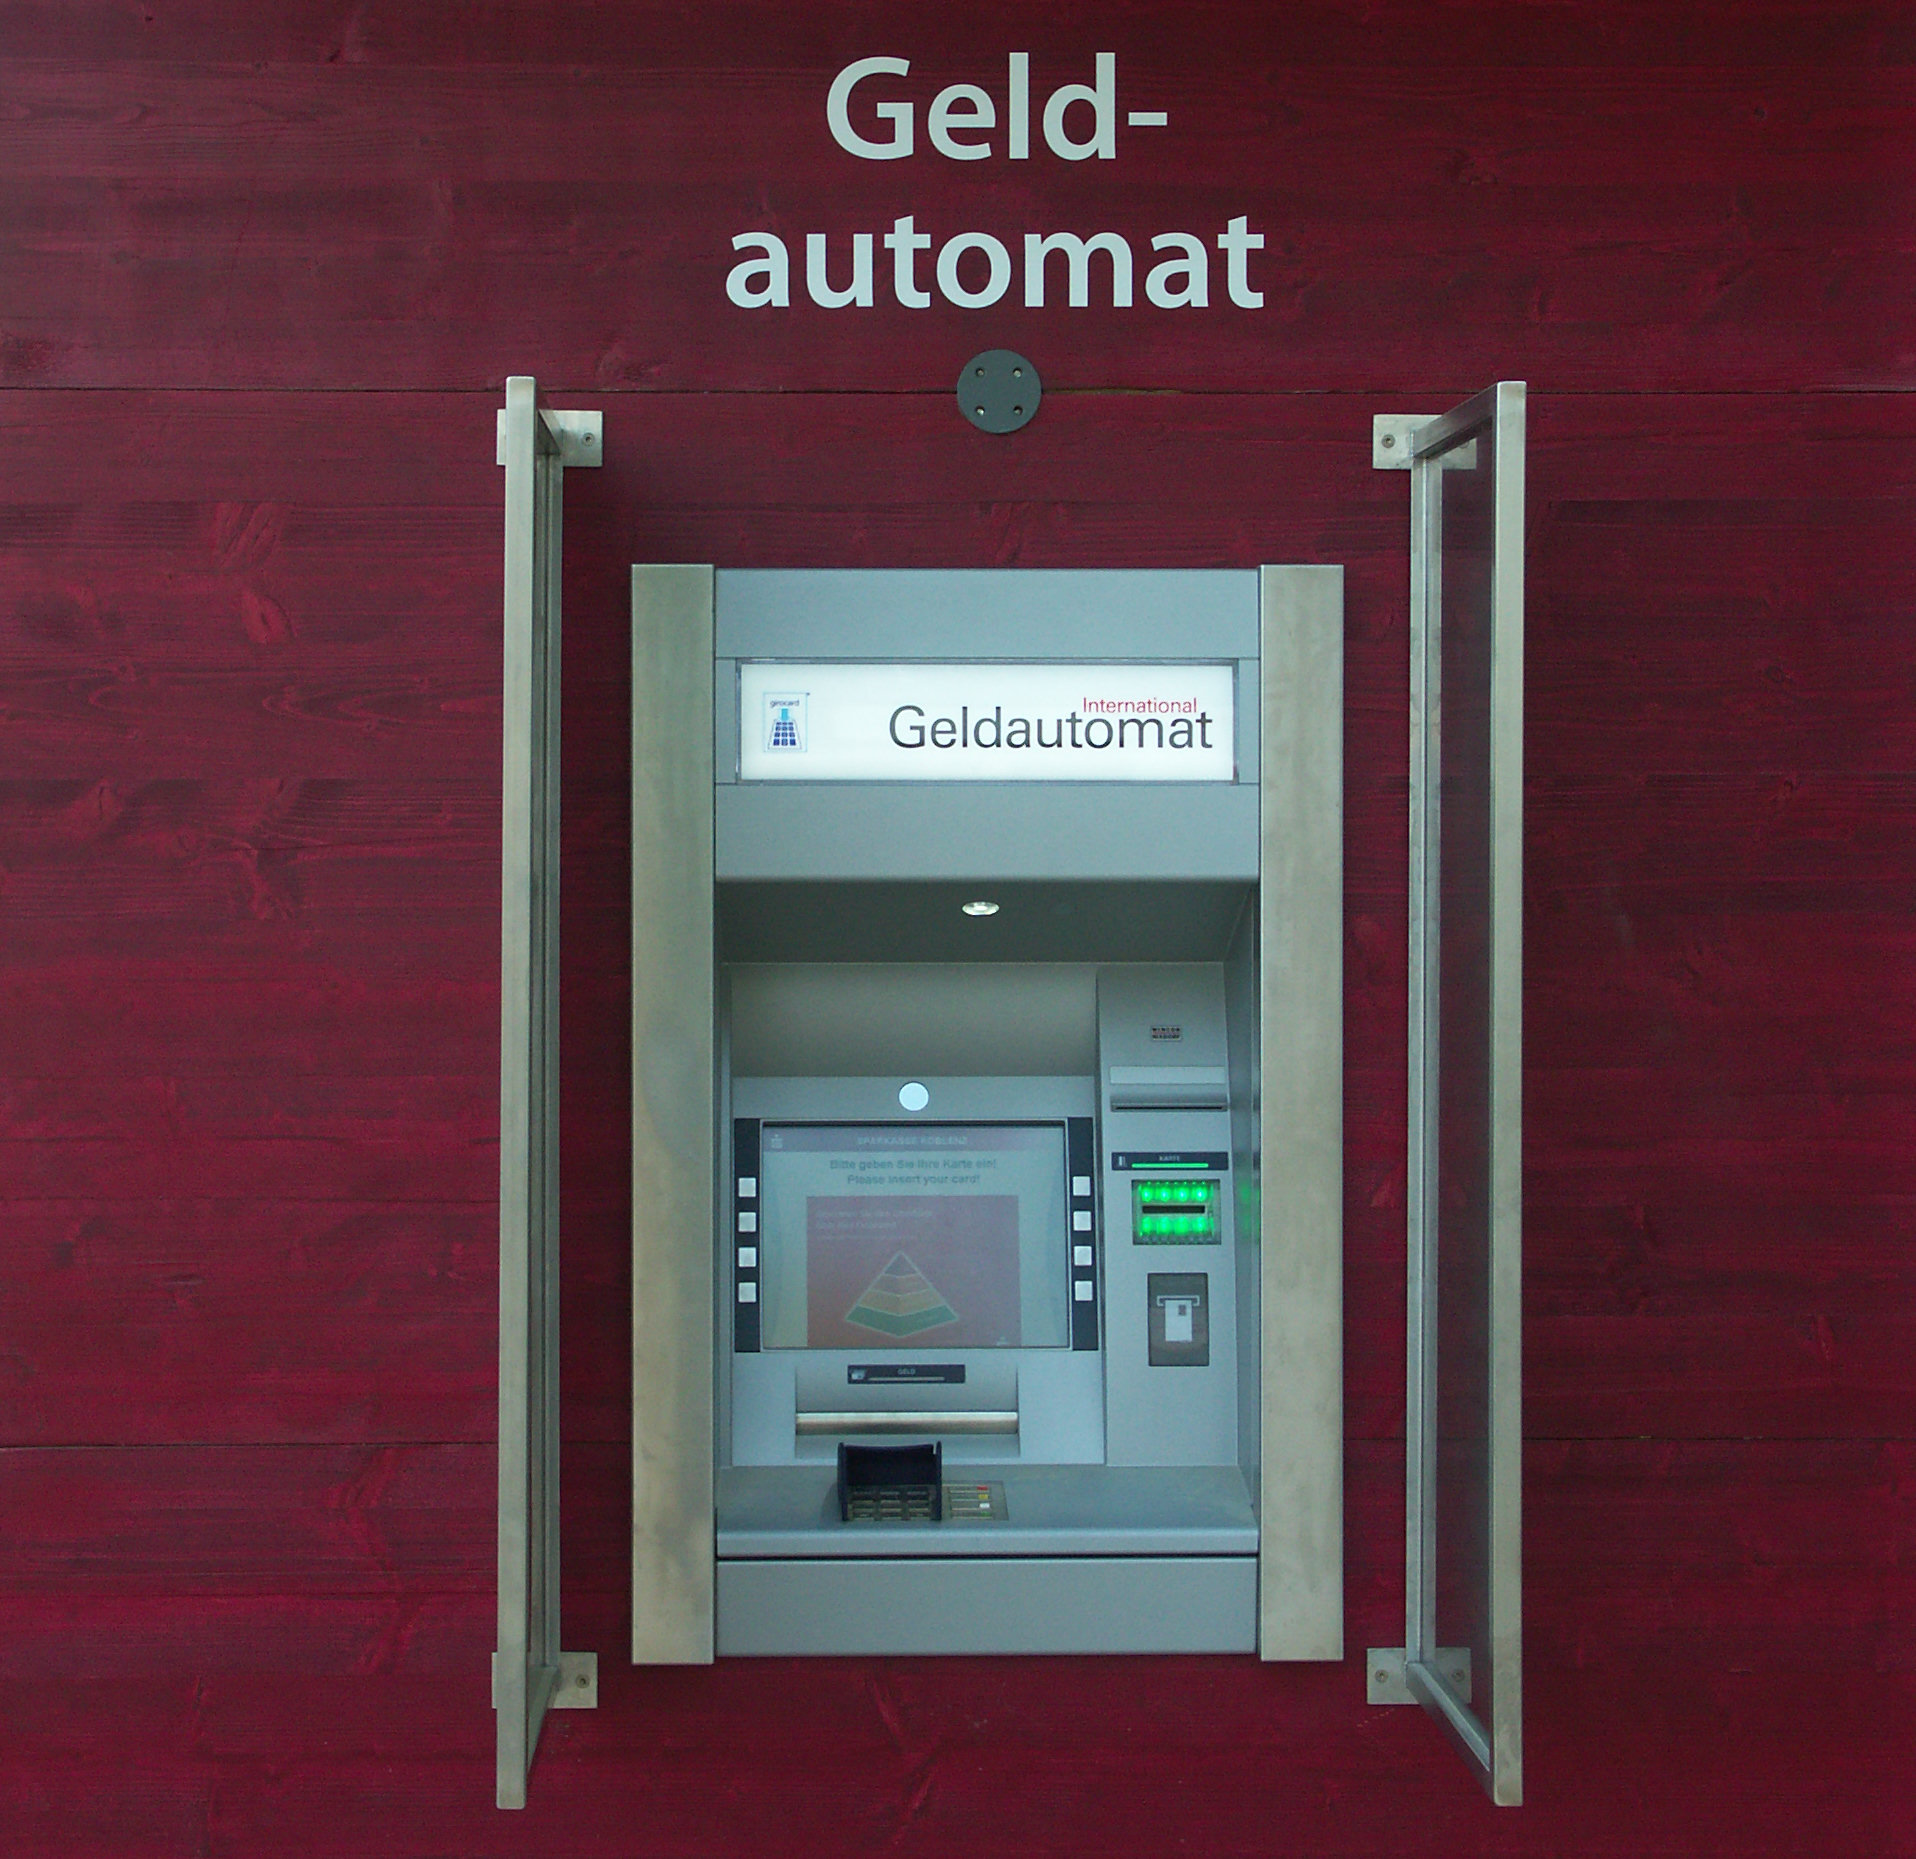
\includegraphics[height=0.7\textheight]{res/wikimedia_geldautomat.jpg}
		\caption{Geldautomat/ATM (or Kontoauszugsautomat/Bank Statement Printer) \newline \tiny \fullcite{wikimedia_image_geldautomat}}
	\end{figure}

	\note{
		Question: Describe the process of withdrawing money on an ATM?
	}
\end{frame}

\begin{frame}{RAII Concept: ATM Example}
	\centering
	\definecolor{gothamYellow}{HTML}{FFCC00} % ignore last FF, LaTeX hex only takes RRGGBB
	\begin{tikzpicture}[
			>=stealth,
			node distance=6cm,
			% Reduce the font size of nodes and labels
			every node/.style = {font=\footnotesize},
			every label/.style = {font=\footnotesize},
			% Specify default state
			every state/.style={thick, minimum size=8mm, align=center},
			% Specify highlighted state
			highlight/.style={draw=gothamYellow, very thick, fill=gothamYellow!30},
		]

		% States
		% > Top row
		\node[state, highlight] (cardInserted) {
			Insert card\\
			(Acquire resource)
		};
		\node[state, right=4cm of cardInserted] (withdraw) {
			Withdraw money/\\bank statements
		};
		% > Bottom row
		\node[state, highlight, below=1cm of withdraw] (returnCard) {
			Return card\\
			(Release resource)
		};
		\node[state, left=4cm of returnCard] (dispense) {
			Dispense money/\\bank statements
		};

		% Transitions
		\draw[->, thick] (cardInserted) -- (withdraw) node[midway, above, align=center] {
			Enter PIN / Authenticate\\
			(Use resource)
		};
		\draw[->, thick] (withdraw) -- (returnCard) node[midway, right, align=center] {};
		\draw[->, thick] (returnCard) -- (dispense) node[midway, above, align=center] {};

	\end{tikzpicture}

	\note{
		Important discovery:
		\begin{itemize}
			\item Card is returned before the \textit{goal} of taking the money is reached
			\item Pattern RAII connects a resource (bank card) to the lifetime of the process to not accidentally forget it
		\end{itemize}
	}
\end{frame}
